\subsection{A First Use-Case:  Comparison of Entropy, Snooze and DVMS}
\label{subsec:first-usecase}
%\AL{Il faudra parler du nombre de migrations qui est egalement une
%  métrique pertinente. Plusieurs algorithms tentent de reduire cette
%  metrique }
%\AL[AL]{Il faudra mettre des snapshots de PajeNG}


% Evaluation of VMPlaceS on Grid'5000: simulations were running on one server.
In this section, we discuss the results of the simulations we
performed on the Entropy, Snooze and DVMS strategies. First, we
present a general study analyzing the violation times as well as the
duration of the computation and reconfiguration phases.
Second, we examine some variants and possible
improvements of Snooze and DVMS that made possible to easily study  thanks to
\vmps.

\subsubsection{Experimental Conditions}
All simulations have been
performed on the Lyon clusters of the Grid'5000 testbed.
Each execution was running on a dedicated server, thus avoiding
interferences between simulations and ensuring reproducibility between
the different invocations.

% Scripts: automation of the deployment, running of simulations and the collect
% of results.

% It enables us to run a large number of simulations, with several variants
% of the scheduling algorithm.

\vmps has been configured in order to simulate an homogeneous
infrastructure of PMs composed of 8 cores, 32~GB of RAM and 1~Gpbs
Ethernet NIC. To enable fair comparison between the three strategies,
the scheduling resolver only considered 7 cores (\ie one was devoted
to run the Snooze LC or the DVMS processes). Dedicating one core for
the host OS and other administrative processes is something which is
rather usual and thus we believe acceptable in our experimental
methodology. Regarding the Virtual Machines, Ten VMs have been
initially launched on each simulated PM. Each VM relied one of the VM
classes previously described in Section \ref{subsec:accuracy} and the
parameters for changing the load were the same ($\lambda$ = Nb
VMs/300, $\mu$ = 60 and $\sigma$ = 20). The stationary state was
reached after 20 min of the simulated time with a global load of 85\%
as depicted in Fig. \ref{fig:load_figure}. To accelerate the
simulations, we have chosen to limit the simulated time to 1800
seconds. It is noteworthy that the consolidation ratio, \ie the number
of VMs per node, has been defined to generate a sufficient number of
violations. We discovered that under a global load of 75\%, our
infrastructure almost did not face VM violations with our selected Gaussian
distribution. Such a result is rather
satisfactory as it can explained why most production DCs target such
an overall utilization rate.\footnote{\url{http://www.cloudscaling.com/blog/cloud-computing/amazons-ec2-generating-220m-annually/}}

We conducted simulations in order to study infrastructures composed of
128, 256, 512 and 1024 PMs, hosting respectively 1280, 2560, 5120 and
10240 VMs. Additional simulated PMs have been provided to execute the
Entropy and Snooze service nodes on distinct nodes. For Snooze, one GM
has been created every 32 LCs (\ie PMs). Entropy and Snooze are
invoked every 30 seconds. Finally, it is noteworthy that no service
node had to be provisioned for DVMS as a DVMS process had been
executed directly on top of the hosting nodes.

In order to cope with real DC conditions, we defined the parameters
for node crashes to simulate a fault on average every 6 months for a
duration of 300 seconds. These values correspond to the Mean Time To
Failure (MTTF) and the Mean Time To Repair (MTTR) of a Google DC
server~\cite[pp. 107-108]{datacenterAsComputer}. We underline that at
the scale we performed our simulations such a crash ratio was not
sufficient to impact the behavior of the scheduling policies.
Dedicated simulations were mandatory to study the influence of node
crashes. However, due to the space limitations, we do not present them
in the article and only gives major trends. Regarding Entropy,
although the lost of the service node can be critic, the failure
probability is so small that the single point of failure issue can be
easily solved by a fail-over approach. Regarding Snooze, the heartbeat
strategy enables the reconstruction of the hierarchy in a relative
short time and thus crashes on service nodes do not significantly
impact the resolution of violations (in our case less than 10 seconds
is mandatory to reorganize the Snooze topology with a 6 seconds
heartbeat mechanism). Finally regarding DVMS, the crash of one node
does not have any impact of the resolution has the composition of the
microcosm is reevaluated immediately.


All configuration files used to perform the discussed simulations can
be downloaded from the \vmps repository.

\subsubsection{General  Analysis}
\label{subsec:general-comparison}

\begin{figure}
\subcapcentertrue
\subfigure[Infrastructure load]{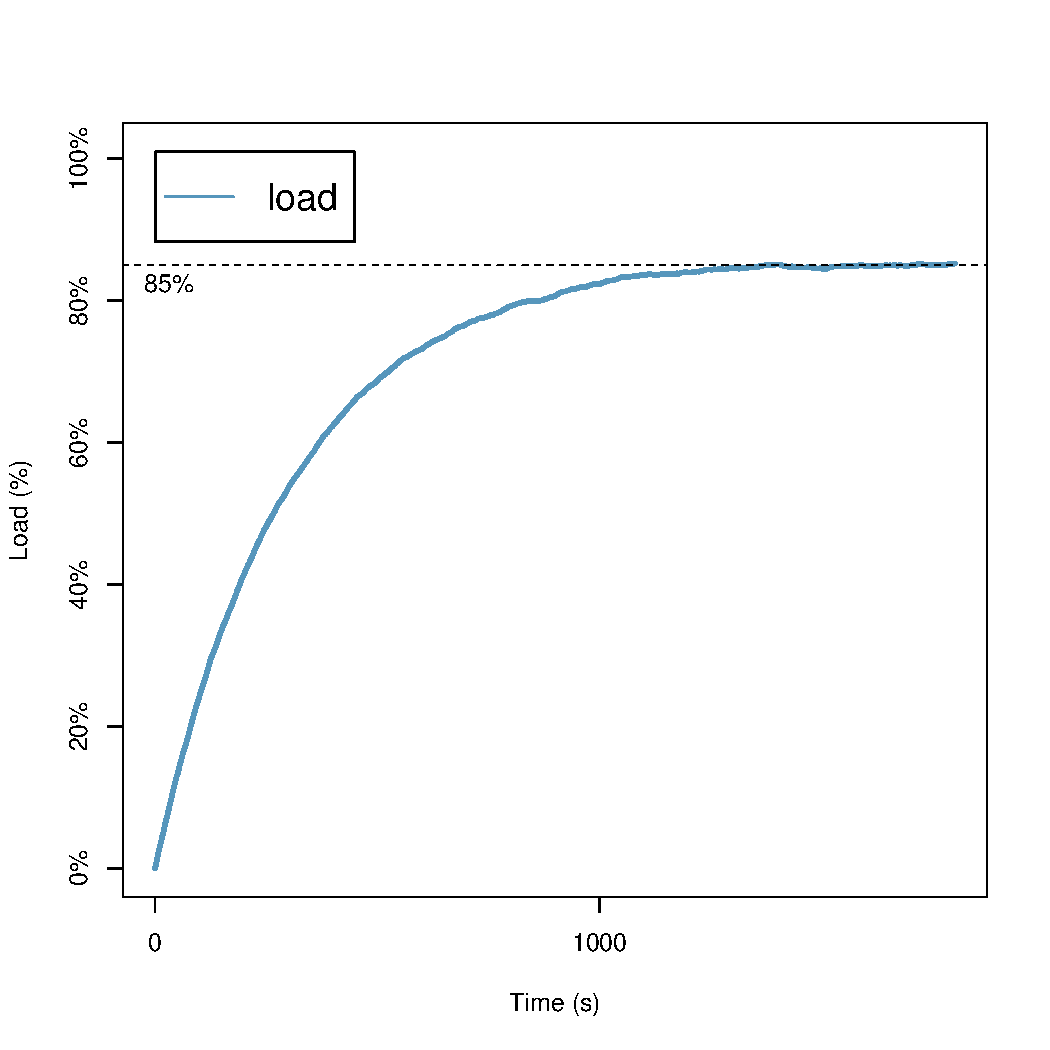
\includegraphics[width=4cm]{./figures/experiments/1024-hierarchical.pdf}\label{fig:load_figure}}
\subfigure[Cumulated Violation Time]{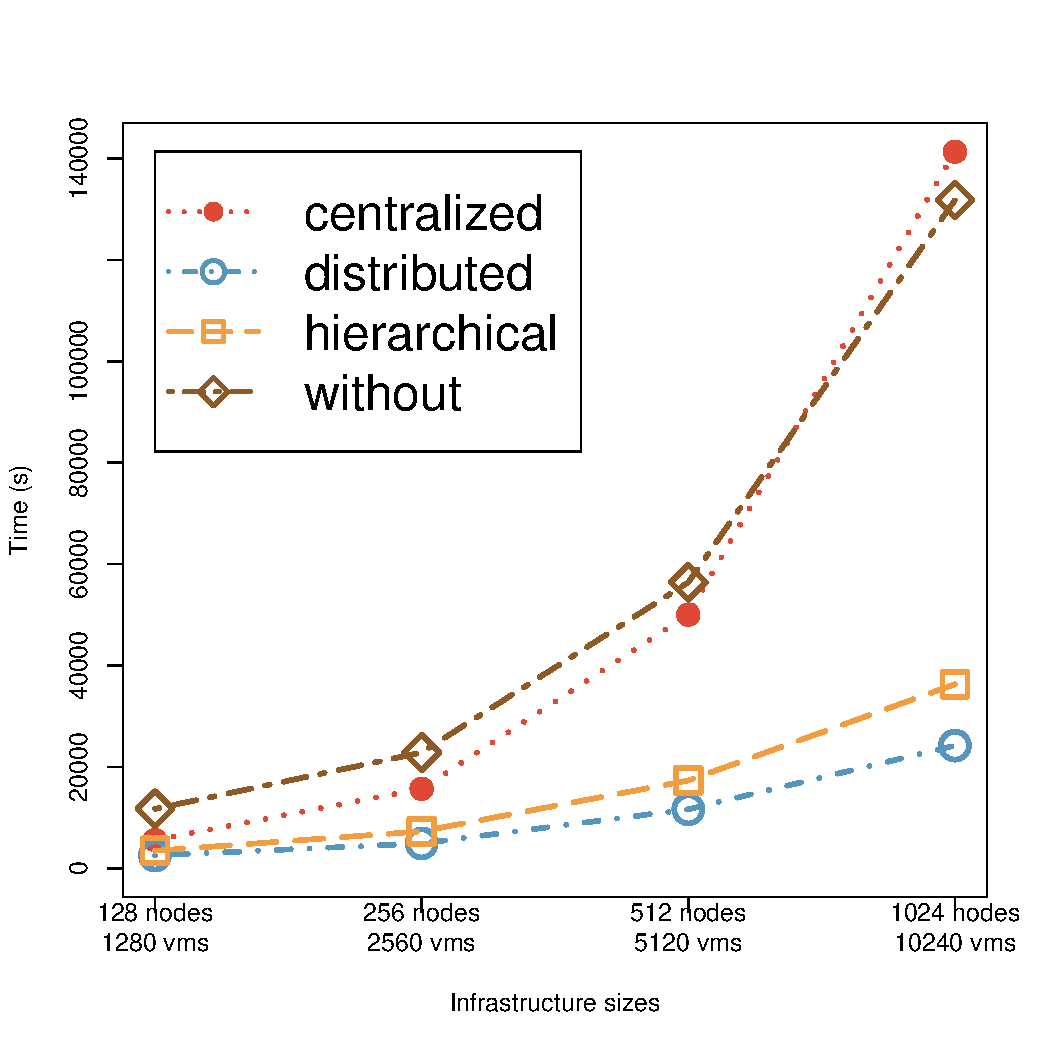
\includegraphics[width=4cm]{./figures/experiments/violation_time.pdf}\label{fig:cumulated_violation}}
\caption{Simulation Results - 10 VMs per node (VM load: $\mu=60$ and $\sigma=20$)}
\label{fig:simulation-overview}
\end{figure}

%%%

% \begin{figure}[ht]
% \centering
% \begin{minipage}[c]{.48\textwidth}
%     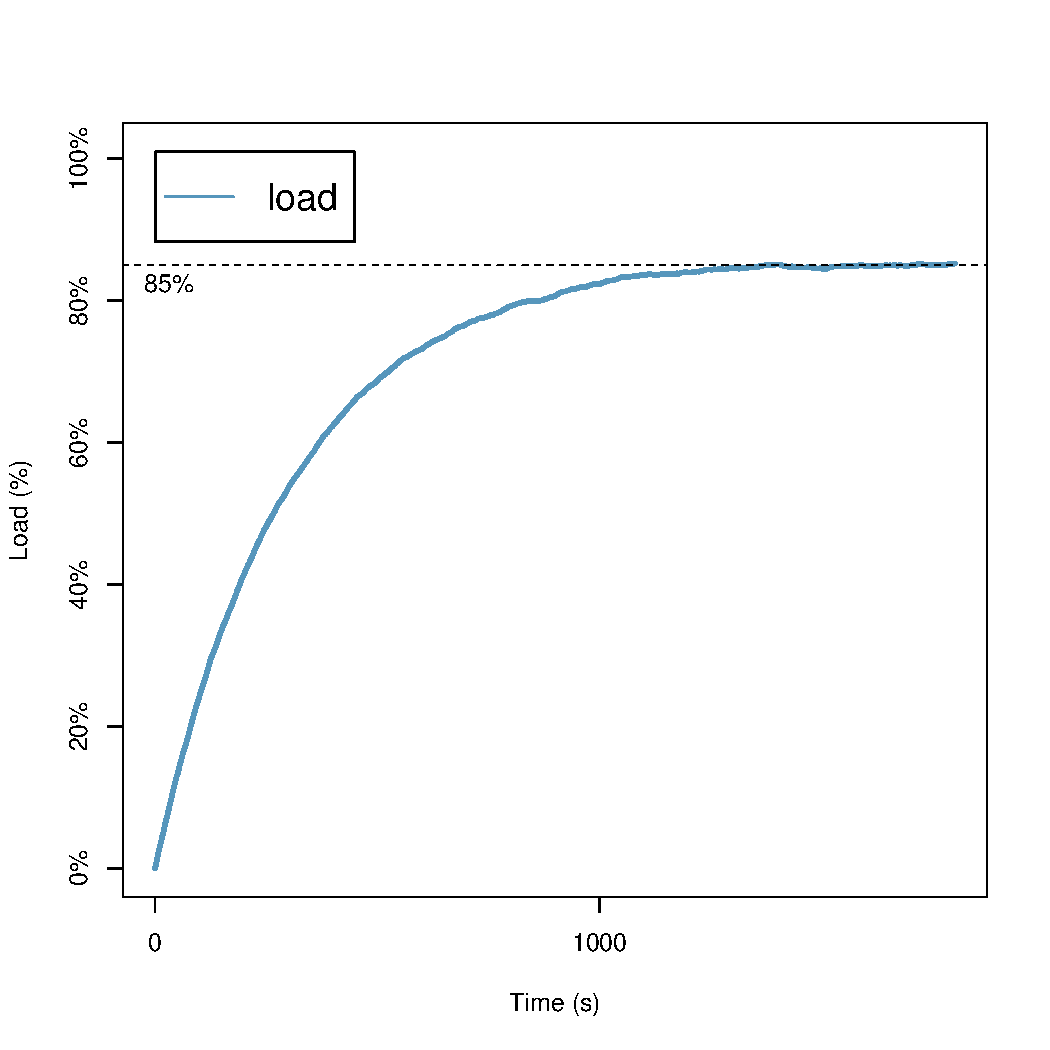
\includegraphics[width=.48\textwidth]{figures/experiments/1024-hierarchical.pdf}
%     \caption{Evolution of the global CPU load}
% \label{fig:load_figure}
% \end{minipage}
% \begin{minipage}[c]{.48\textwidth}
%      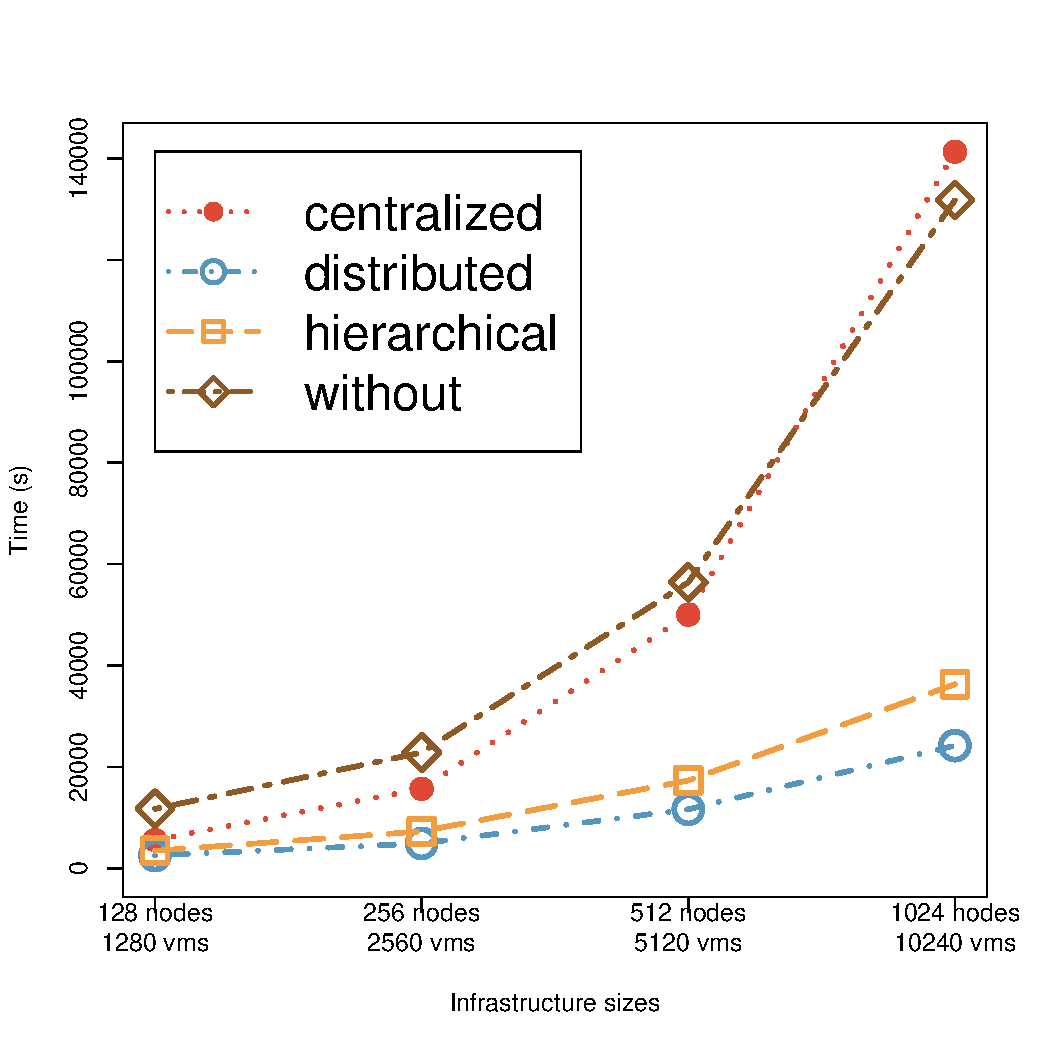
\includegraphics[width=.48\textwidth]{figures/experiments/violation_time.pdf}
%      \caption{Cumulated Violation Duration}
% \label{fig:cumulated_violation}
% \end{minipage}
% \end{figure}

%To enable a fair comparison of several scheduling algorithms, the simulations is
%associated with a workload simulator which simulates a virtual workload in each
%simulated virtual machines, thus enabling the study of the behaviour of the
%simulated algorithms.
%The figure \ref{fig:load_figure} illustrates the global load.
%To accelerate the simulations, we have chosen
%parameters that cause the workload to reach a stationary phase after 1200
%seconds of simulations, thus enabling us to limit the simulation duration to
%1800 seconds.

Fig.~\ref{fig:cumulated_violation} presents the cumulated violation
time for each placement policy while
Tables~\ref{table:detailed_violation_time},
\ref{table:detailed_computation_time} and
\ref{tab:detailed_reconf_time} give more details by presenting the
mean and the standard deviations of the duration of, respectively, the
violations, the computation and reconfiguration phases. As
anticipated, the centralized approach did not scale and became almost
counterproductive for the largest scenario in comparison to a system
that did not use any dynamic scheduling strategy. The more nodes Entropy has to
monitor, the less efficient it is on both the computation and
reconfiguration phases. Regarding the computation, the VMPP is a
NP-Hard problem and thus it is not surprising that it takes more time
to resolve larger problems. Regarding the reconfiguration, as Entropy
has to solve much more violations simultaneously, the reconfiguration plan
is more complex for large scenarios, including several migrations
coming from and going to the same nodes. Such reconfiguration plans
are non optimal as they increase the bottleneck effects at the network
level of each involved PM. Such a simulated result is valuable as it confirms
that reconfiguration plans should avoid as much as possible such
manipulations.

% \begin{table}[ht]
% \centering
%     {\scriptsize \begin{tabular}{|P{10mm}@{\:}||@{\:}c@{\:}|@{\:}c@{\:}|@{\:}c@{\:}||@{\:}c@{\:}|@{\:}c@{\:}|@{\:}c@{\:}|}
%       \thickhline
%       \textbf{Infrastructure Size}
%         & \multicolumn{4}{c@{\:}||@{\:}}{\textbf{Algorithm}}
%           \Tstrut \\
%          \hfill & ~Without~ & ~Centralized~ & ~Hierarchical~ & Distributed \Bstrut \\
%       \thickhline
%         128 nodes  & 79.20 $\pm$  89.94 & 21.26 $\pm$ 13.55 & 21.07 $\pm$ 12.32 &   9.55 $\pm$ 2.57 \\
%         256 nodes  & 70.86 $\pm$  87.56 & 40.09 $\pm$ 24.15 & 21.45 $\pm$ 12.10 &   9.58 $\pm$ 2.51 \\
%         512 nodes  & 65.63 $\pm$  65.56 & 55.63 $\pm$ 42.26 & 24.54 $\pm$ 16.95 &   9.57 $\pm$ 2.67 \\
%         1024 nodes & 85.90 $\pm$ 101.51 & 81.57 $\pm$ 86.59 & 29.01 $\pm$ 38.14 & \:9.61 $\pm$ 2.54
%       \Rstrut  \\ \hline
%       \thickhline
%   \end{tabular} }
% \caption{Means $\pm$ Std deviations of violation durations.}
% \label{table:detailed_violation_time}
% \end{table}

\begin{table}[ht]
\centering
    {\scriptsize \begin{tabular}{|P{27mm}@{\:}||@{\:}c@{\:}|@{\:}c@{\:}|@{\:}c@{\:}|}
      \thickhline
      \textbf{Infrastructure Size}
        & \multicolumn{3}{c@{\:}|}{\textbf{Algorithm}}
          \Tstrut \\
         \hfill  & ~Centralized~ & ~Hierarchical~ & Distributed \Bstrut \\
      \thickhline
        128 nodes   & 21.26 $\pm$ 13.55 & 21.07 $\pm$ 12.32 &   9.55 $\pm$ 2.57 \\
        256 nodes   & 40.09 $\pm$ 24.15 & 21.45 $\pm$ 12.10 &   9.58 $\pm$ 2.51 \\
        512 nodes   & 55.63 $\pm$ 42.26 & 24.54 $\pm$ 16.95 &   9.57 $\pm$ 2.67 \\
        1024 nodes  & 81.57 $\pm$ 86.59 & 29.01 $\pm$ 38.14 & \:9.61 $\pm$ 2.54
      \Rstrut  \\ \hline
      \thickhline
  \end{tabular} }
\caption{Duration of violations ($Med \pm \sigma$)}
\label{table:detailed_violation_time}
\end{table}

\begin{table}[ht]
\centering
    {\scriptsize \begin{tabular}{|P{27mm}@{\:}||@{\:}c@{\:}|@{\:}c@{\:}|@{\:}c@{\:}|}
      \thickhline
      \textbf{Infrastructure Size}
        & \multicolumn{3}{c@{\:}|}{\textbf{Algorithm}}
          \Tstrut \\
         \hfill  & ~Centralized~ & ~Hierarchical~ & Distributed \Bstrut \\
      \thickhline
        128 nodes   &  3.76 $\pm$  7.43 &  2.52 $\pm$  4.63 &   0.29 $\pm$ 0.03 \\
        256 nodes   &  7.97 $\pm$ 15.03 &  2.65 $\pm$  4.69 &   0.25 $\pm$ 0.02 \\
        512 nodes   & 15.71 $\pm$ 29.14 &  2.83 $\pm$  4.98 &   0.21 $\pm$ 0.01 \\
        1024 nodes  & 26.41 $\pm$ 50.35 &  2.69 $\pm$  4.92 & \:0.14 $\pm$ 0.01
      \Rstrut  \\ \hline
      \thickhline
  \end{tabular} }
\caption{Duration of computations ($Med \pm \sigma$)}
\label{table:detailed_computation_time}
\end{table}

\begin{table}[ht]
\centering
    {\scriptsize \begin{tabular}{|P{27mm}@{\:}||@{\:}c@{\:}|@{\:}c@{\:}|@{\:}c@{\:}|}
      \thickhline
      \textbf{Infrastructure Size}
        & \multicolumn{3}{c@{\:}|}{\textbf{Algorithm}}
          \Tstrut \\
         \hfill  & ~Centralized~ & ~Hierarchical~ & Distributed \Bstrut \\
      \thickhline
        128 nodes   & 10.34 $\pm$  1.70 &  10.02 $\pm$  0.14 &   10.01 $\pm$ 0.11 \\
        256 nodes   & 10.26 $\pm$  1.45 &  10.11 $\pm$  0.83 &   10.01 $\pm$ 0.08 \\
        512 nodes   & 11.11 $\pm$  3.23 &  10.28 $\pm$  1.50 &   10.08 $\pm$ 0.82 \\
        1024 nodes  & 18.90 $\pm$  7.57 &  10.30 $\pm$  1.60 & \:10.04 $\pm$ 0.63
      \Rstrut  \\ \hline
      \thickhline
  \end{tabular} }
\caption{Duration of reconfigurations ($Med \pm \sigma$).}
\label{tab:detailed_reconf_time}
\end{table}

Regarding Snooze, although the performances are better than the
Entropy ones, we may erroneously conclude that the hierarchical
approach is not competitive with respect to the distribued strategy at
the first sight. However, diving into details, we can see that both
the computation and reconfiguration phases are almost constants
(around 3 seconds and 10 seconds) and not so far from the DVMS values,
especially for the reconfiguration phase, which is predominant. These
results can be easily explained: the centralized policy adresses the
VMPP by considering all nodes at each invovation, while the
hierarchical and the distributed algorithms divide the VMPP into sub
problems, considering smaller numbers of nodes (32~PMs in Snooze and
4 in average with DVMS). To clarify the influence of the group size on
the Snooze performances, \ie the ratio of LCs attached to one GM, we
performed additional simulations aiming at investigating whether a
smaller group size can lead to similar performances of DVMS. We
higlight that the use of \vmps eased such a study as it has consisted
to simply relaunch the previous simulation with a distinct
assignment.


\begin{figure*}
\subcapcentertrue
\subfigure[Total Violation Times]{
  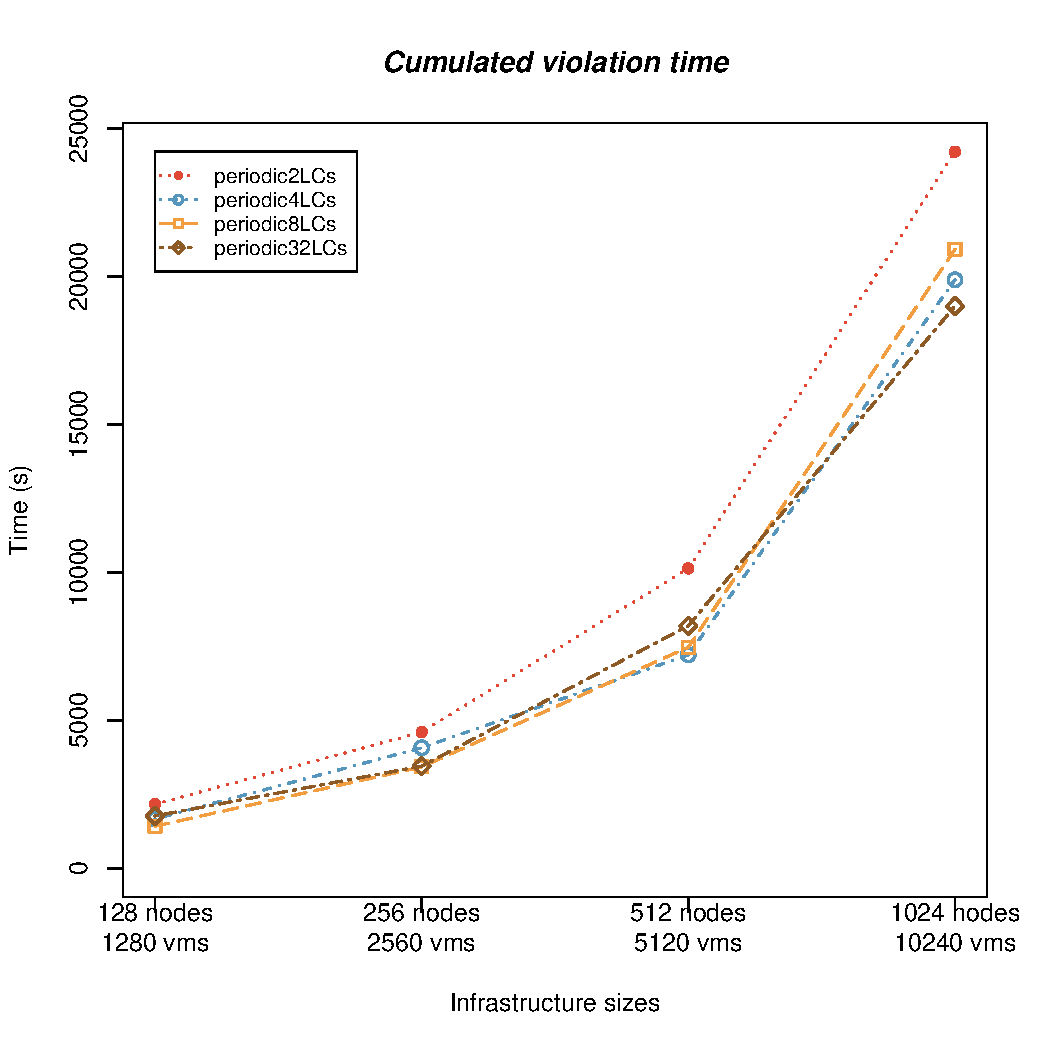
\includegraphics[width=.32\textwidth]{figures/groupSizes-violationTime.pdf}
  \label{fig:groupSizesViolationTime}}
\begin{minipage}{.66\textwidth}\centering
  \vspace*{-4.5cm}
\subfigure[No.\ of Failed Reconfigurations]{
    {\scriptsize \begin{tabular}[b]{|r@{\:}||@{\:}r@{\:}|@{\:}r@{\:}|@{\:}r@{\:}|@{\:}r@{\:}|}
      \thickhline
      \textbf{Infra.\ Size~~}
        & \multicolumn{ 4 }{c@{\:}|}{\textbf{No.\ of failed reconfigurations}}
          \Tstrut \\
         \hfill &  ~2 LCs~ & ~4 LCs~ & ~8 LCs~ &  ~32 LCs~  \Bstrut \\
      \thickhline

        128~~~~~~~ &  19~ & 0~ & 0~ & 0~ \\
        256~~~~~~~ &  29~ & 0~ & 0~ & 0~ \\
        512~~~~~~~ &  83~ & 1~ & 0~ & 0~ \\
       1024~~~~~~~ & 173~ & 7~ & 0~ &  0
      \Rstrut  \\ \hline
      \thickhline
  \end{tabular} }
  \label{fig:groupSizesReconfigFail}
  }
\subfigure[Means $\pm$ Std deviations of computation durations.]{
    {\scriptsize \begin{tabular}[b]{|r@{\:}||@{\:}c@{\:}|@{\:}c@{\:}|@{\:}c@{\:}|@{\:}c@{\:}|}
      \thickhline
      \textbf{Infra.\ Size~~}
        & \multicolumn{ 4 }{c@{\:}|}{\textbf{Algorithm}}
          \Tstrut \\
         \hfill &  ~2 LCs~ & ~4 LCs~ & ~8 LCs~ & 32 LCs  \Bstrut \\
      \thickhline

        128~~~~~~~ &   0.16 $\pm$   1.23 &   0.34 $\pm$   1.81 &   0.58 $\pm$   2.40 &   2.53 $\pm$   4.62  \\
        256~~~~~~~ &   0.18 $\pm$   1.31 &   0.42 $\pm$   1.99 &   0.66 $\pm$   2.50 &   2.65 $\pm$   4.69  \\
        512~~~~~~~ &   0.15 $\pm$   1.20 &   0.33 $\pm$   1.78 &   0.67 $\pm$   2.54 &   2.83 $\pm$   4.98  \\
       1024~~~~~~~ &   0.19 $\pm$   1.37 &   0.42 $\pm$   2.02 &   0.89 $\pm$   2.90 &   ~2.69 $\pm$   4.91

      \Rstrut  \\ \hline
      \thickhline
  \end{tabular} }
  \label{fig:groupSizesComputationTime}
  }
\end{minipage}
\caption{Hierarchical placement: influence of varying group sizes}
\label{fig:snoozeGroupSizes}
\end{figure*}

\paragraph{Varying group sizes}

Figure \ref{fig:snoozeGroupSizes} presents the simulated values
obtained for scenarios with 2,~4,~8 and 32~LCs per GM for four
infrastructure sizes. The overall performance (\ie cumulated violation
time), shown in Fig.~\ref{fig:groupSizesViolationTime}, shows that
2~LCs per GM result in significantly higher violation times. All other
group sizes yield violation times that are relatively close, which
indicates that a small group size does not help much in
resolving violations faster.

The relatively bad performance of the smallest group size can be
explained in terms of the number of failures of the reconfiguration
process, that is, overloading situations that are discovered but
cannot be resolved because the GM managing the overloaded VM(s) did
not dispose of enough resources, see
Table~\ref{fig:groupSizesReconfigFail}. Groups of 2~LCs per GM are
clearly insufficient at our load level (60\% mean, 20\% stddev).
Failed reconfigurations are, however, already very rare in the case of
4~LCs per GM and do not occur at all for 8~and 32~LCs per GM. This is
understandable because the load is statistically evenly distributed
among the LCs and tthe load profile we evaluated only rarely results
in many LCs of a GM to be overloaded. Violations can therefore be
resolved even in the case of a smaller number (4) LCs available for
load distribution.

Conversely, we can see that the duration of the overall
reconfiguration phases decreases strongly along with the group
size. It reaches a value close to the computation times of DVMS for a
group size of 4-LCs per GM, see Fig.~\ref{fig:groupSizesComputationTime}.
We thus cannot minimize computation times and violation times by
reducing the number of LCs because larger group sizes are necessary to
resolve overload situations if the VM load gets higher.  Once again,
this information is valuable as it will help researchers to design new
algorithms favoring the automatic discovery of the optimal subset of
nodes capable to solve violations under for given load profiles.

In contrast, DVMS resolves this trade-off by construction because of its
automatic and dynamic choice of the partition size necessary to handle
an overload situation.
% Although DVMS selects naively its neighborhood without
% considering whether it is relevant or note, we can consider that DVMS
% is one of such advanced algorithm.


% \begin{figure}[ht]
% \begin{center}
%     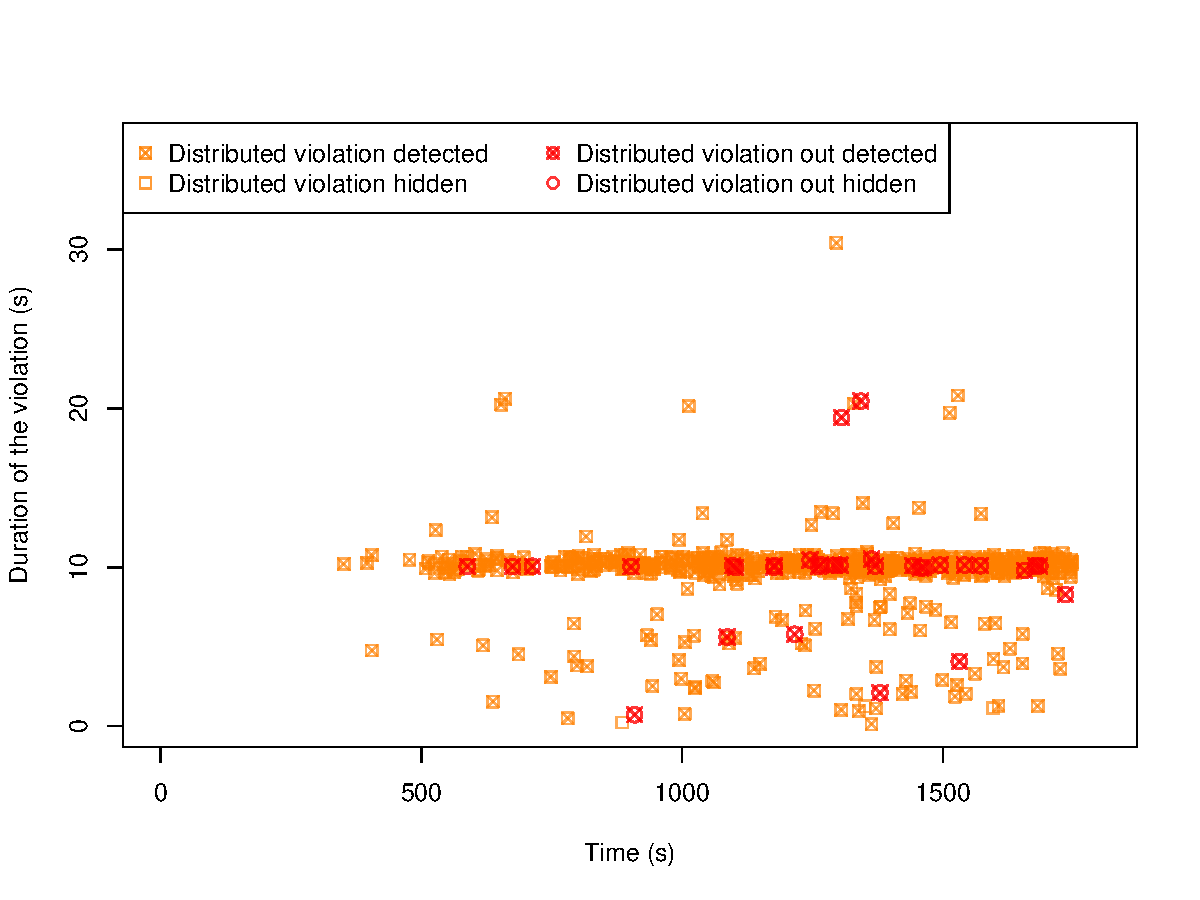
\includegraphics[width=.85\linewidth]{figures/experiments/clouds-1024-distributed.pdf}
%     \caption{Details of violations duration occuring during simulation (10240 VMS).}
% \end{center}
% \label{fig:violation_clouds_dvms_1024}
% \end{figure}

% \begin{figure}[ht]
% \begin{center}
%     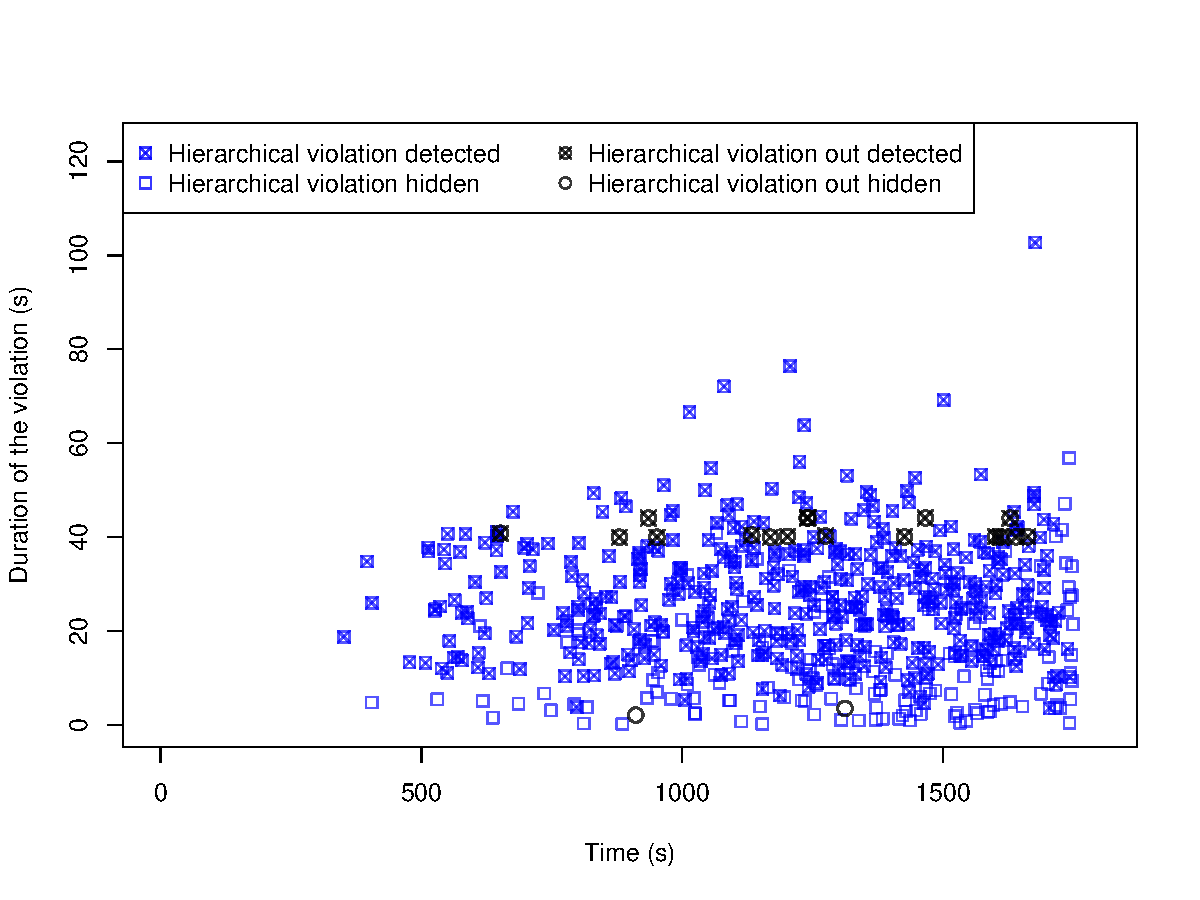
\includegraphics[width=.85\linewidth]{figures/experiments/clouds-1024-hierarchical.pdf}
%     \caption{Details of violations duration occuring during simulation (10240 VMS).}
% \end{center}
% \label{fig:violation_clouds_snooze_1024}
% \end{figure}


\begin{figure}[ht]
\begin{center}
    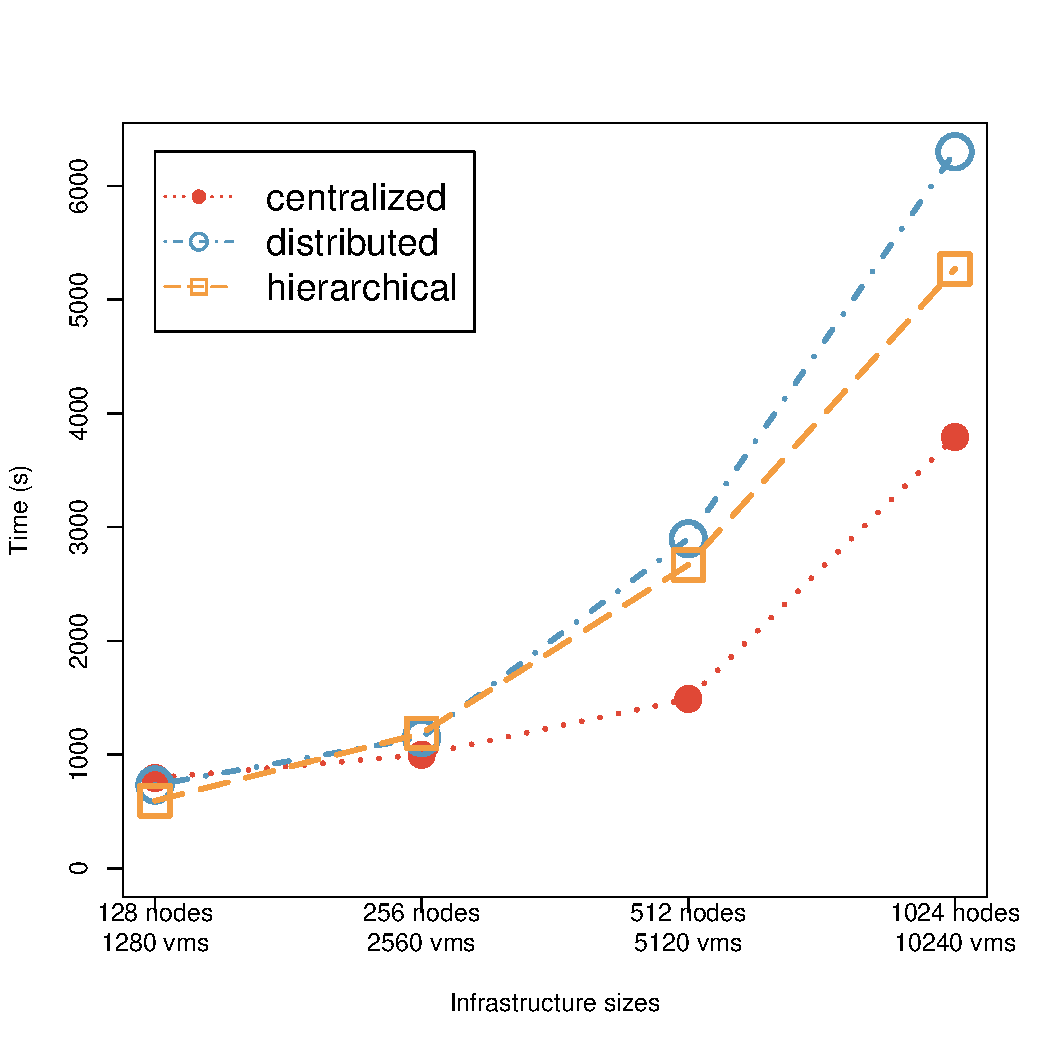
\includegraphics[width=.65\linewidth]{figures/experiments/migration_time.pdf}
    \caption{Cumulated migration time.}
\end{center}
\label{fig:cumulated_migration_time}
\end{figure}

\begin{figure}[ht]
\begin{center}
    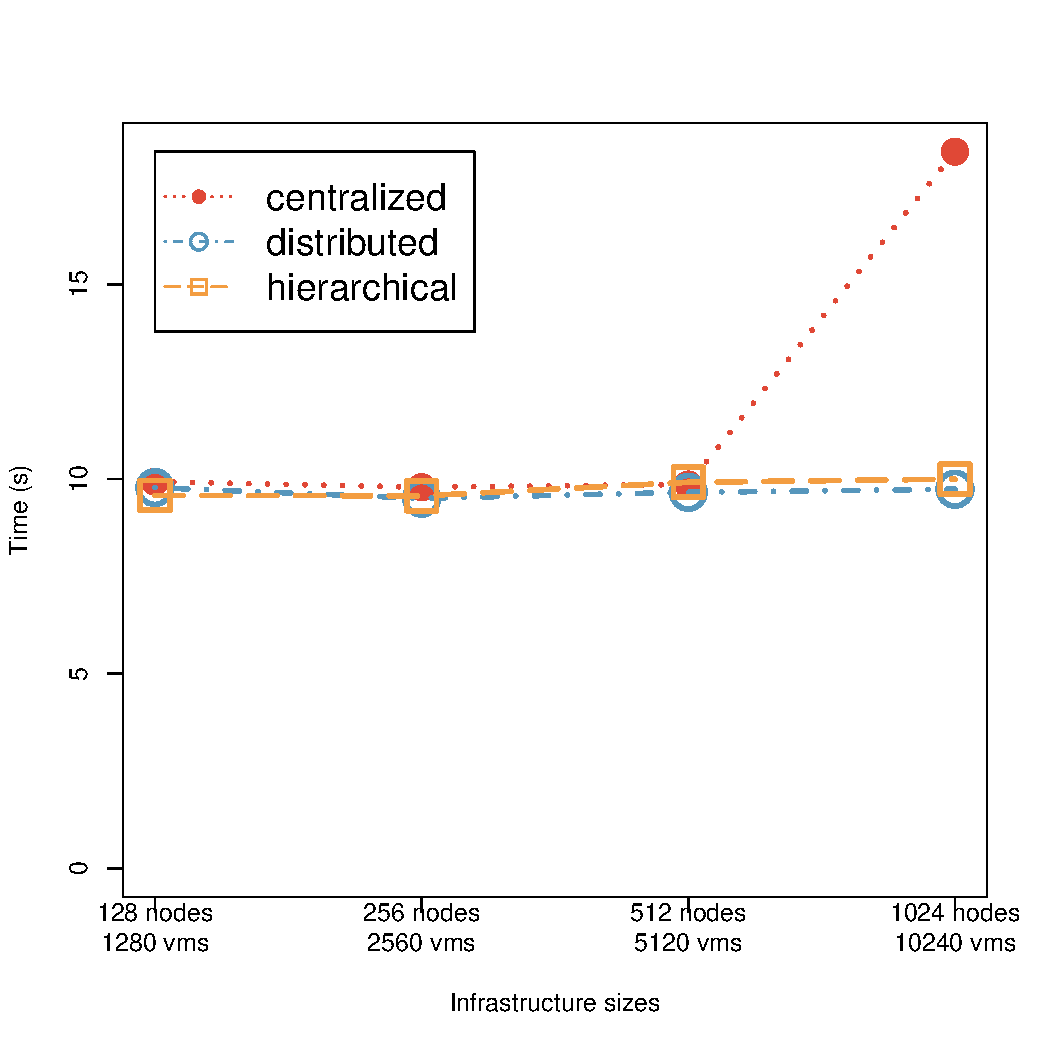
\includegraphics[width=.65\linewidth]{figures/experiments/migration_avg_duration.pdf}
    \caption{Average duration of a migration.}
\end{center}
\label{fig:avg_migration_time}
\end{figure}

% * migration_time.pdf:
% - On the other hand centralised do less migrations: it can be explained by its
%   lack of reactivity.
% - Distributed and Hierarchical have similar results, even if hierarchical do
%   less migrations.


Another important metric when performing dynamic relocations is
related to the migration overhead on the network but also on the
workload running inside each VM. Hence it is important to understand
how VM Placement algorithms deal with such a concern.
\AL[AL]{finalized that part with the following paragraph}

Figure \ref{fig:cumulated_migration_time} describes the cumulated migrations number for
each strategy: the distributed algorithm spend more time
on migrating VMs, followed by the hierarchical scheduler. It is noticeable that
the centralized scheduler performes spend less time in migration of VMs. Thanks
to figure \ref{fig:avg_migration_time}, we can see that the average duration
of a migration increases dramatically with the centralized policy at large scale
(10240 VMs), while it remains stable with the distributed and hierarchical
schedulers. This is due to the fact that the unique node invocking Entropy does
not find the best reconfiguration in an adequate time, and must confine itself
to a non optimal reconfiguration. These non optimal reconfigurations usually
contain several migrations to the same nodes, thus leading to network congestion
and increasing the average migration duration.


% \subsubsection{Hierarchical VM placement: evaluation of GM sizes}

% We have also explored the use of \vmps in order to explore the
% principal parameters of different VM placement algorithms. In the
% remainder of this section we report of one example, the influence of
% the cluster size, \ie the ratio of LCs to GMs, on hierarchical VM
% placement. For these experiments, VM reconfigurations have been
% calculated and applied periodically every 30 secs.

% {\scriptsize \begin{tabular}{|P{25mm}@{\:}||@{\:}c@{\:}|@{\:}c@{\:}|@{\:}c@{\:}||@{\:}c@{\:}|@{\:}c@{\:}|@{\:}c@{\:}|}
%     \thickhline
%     \textbf{Algorithm}
%       & \multicolumn{3}{c@{\:}||@{\:}}{\textbf{Reconf.\ time (s)}}
%       & \multicolumn{3}{c@{\:}|}{\textbf{Violation time (s)}}
%         \Tstrut \\
%        \hfill\#LCs  & ~128~ & ~256~ & 512 & ~~128~~ & ~~256~~ & 512 \Bstrut \\
%     \thickhline
%       ~8 LC/GM      & 4680 & 10755 & 22022 & 1423 & 3429 & 7470 \\
%       32 LC/GM      & 16533 & 33376 & 73623 & 1770 & 3453 & \:8196
%     \Rstrut  \\ \hline
%     \thickhline
% \end{tabular} }

% The table above shows some of the corresponding results for
% experiments on 128, 256 and 512 LCs. The results show that the total
% reconfiguration time (cumulative over all nodes) is significantly
% higher for the configuration of 32~LCs per GM than for 8~LCs per
% GM. This can be explained because the computation of a reconfiguration
% plan for 32~LCs is much costlier than for 8. The cumulative violation
% times of both algorithms are, however, relatively close, which
% indicates that no algorithm is clearly better in resolving
% violations. This is understandable because the load is statistically
% evenly distributed among the LCs. Furthermore, the load profile we
% evaluated only rarely results in many LCs of a GM to be overloaded:
% violations can therefore be resolved even in the case of a smaller
% number of 8~LCs available for load distribution.

% \subsubsection{Fault Tolerance}
% %\AL[JP]{perform an experiment on Snooze and DVMS with fault
% %  periodicity of a crash on average every 160 seconds, corresponding
% %  to a 6 month fault in a DC of 1000 }

% However, we underline that at the scale we
% performed our simulations, the number of crashes was mostly null and
% dedicated simulations were mandatory to study the impact of node
% crashes on the difference strategies.
% \AL[all]{We can maybe add few sentences on that point. Something like:
% Due to the space limitations these results are not discussed in the
% present article. However, we highlight that due to the rather short
% time to reconstruct the Snooze service nodes topology in case of a
% failures. Node crashes does not have an significant impact of the
% violation time resolution. When a GL or a GM crashes, LCs are correcly
% reassigned in less than 10 seconds.}

\AL[MS,AL]{TODO find the best place to add the following paragraph}
To conclude, although the simulations discussed in this article are
limited to 10K VMs, we succeeded to conduct DVMS simulations including
up to 8K~PMs/80K~VMs in a bit less than two days. We did not present
such results to the paper because it was not possible to run a
sufficient number of Snooze simulations at such scale. The Snooze
protocol being more complex than the DVMS one (heartbeats,
consensus,~\ldots), the time to perform a similar experiment is much
more important (around 7 days). The time-consuming portions of the
code are related to \sg internals such as \texttt{sleep} and
\texttt{send/recv} calls. Hence, we have contacted the \sg core
developers in order to investigate how we can reduce the required time
to perform such advanced simulations.




